% (M5-M24) Leader: NCSR "D"
% CeADAR, UPC, ATOS, EVIDEN, FDI, INRIA, ARCADA, use case partners

\subsection{Introduction}

This task will implement a range of methods for automatically
annotating data with respect to quality or possible unreliability.

We will explore anomaly detection and other noise detection methods
that will allow identifying biased, noisy, inconsistent, or in general
low-quality data, as well as data maliciously manipulated to
contaminate the model during training. For these purposes, data
augmentation techniques based on adversarial machine learning methods
(such as controlled noise contamination of the dataset) will be used.

\subsection{Autoencoding}

\subsubsection{Problem Statement}

Our research focuses on the automatic annotation of EEG signals collected from the Bitbrain headband, which uses two EEG channels synchronized with medical-grade EEG devices. These signals are annotated by three experts, with each 30-second segment classified into one of five sleep stages: Wake, N1, N2, N3, and REM. Each sleep stage corresponds to unique patterns of brain activity, such as slow eye movements, sleep spindles and waveforms.

Manually annotating such large amounts of data is inefficient and impractical. Our goal is to build machine learning models capable of predicting sleep stages from EEG signals, eliminating the need for human annotators. To achieve reliable model performance, it is crucial that the training data consists of high-quality signals. This means that the dataset must be free from anomalies, noise, and outliers, as these can negatively impact the training process. During our efforts towards this goal, we encountered a key challenge, regarding the size of our dataset. With recordings from 128 nights, each consisting of thousands of 30-second EEG segments, the dataset ends up having millions of time steps that must be processed during training. Since brain signals typically show low variability, larger datasets are often necessary for models to learn meaningful patterns. However, training on such large datasets is computationally expensive and, when resources are limited, it can become nearly impossible.

\subsubsection{Proposed Methodology}

To address this issue, we propose encoding the EEG signals into a latent representation to reduce their dimensionality. This method creates smaller embeddings from the original signals, making the data more manageable for further processing and model training. For the transformation to be successful, the embeddings must preserve the key characteristics of the original signals without losing important information.

To achieve this, we train an autoencoder and use the encoder component of the model to transform the signals into a lower-dimensional representation. Autoencoders are designed to reconstruct data from a lower-dimensional representation. In our case, if the decoder performs well in reconstructing the original signals, it indicates that the encoder has effectively captured the critical features of the data. Therefore, using the latent representation provided by the encoder, will not result in significant loss of important information. We design both an LSTM-based autoencoder and an attention-based autoencoder to compare their performance. By evaluating both architectures, we aim to determine which one is more effective at capturing the essential features of the data while reducing dimensionality.

\subsubsection{Experimental Setup}


Our dataset consists of EEG recordings from 128 nights, where each night is split into multiple 30-second segments. These segments contain 7680 samples each. For our experiments, we use only part of the dataset for training and evaluation, specifically: 43 nights for training, 3 for validation, and 10 for testing.

We handle missing and ambiguous data by removing any samples that the expert annotators could not agree on (i.e., samples where the class label has a value of -1) as well as rows containing NaN values.

In terms of normalization, due to the low variability and the presence of extreme outliers in the EEG signals, we adopt a robust normalization approach. Instead of using the mean and standard deviation, which are sensitive to outliers, we rely on the median and interquartile range (IQR). Our normalization method scales the data based on statistics computed across the entire dataset, rather than on a per-batch basis, as the statistics remained consistent across the full dataset.
%
\begin{equation}
x_{\text{norm}} = \frac{x - \text{median}(x)}{\text{IQR}(x)} \label{eq:robust_norm}
\end{equation}
%
where $x$ represents the values of a particular feature, $\text{median}(x)$ is the median value of the feature, and $\text{IQR}(x)$ is the interquartile range, which measures the spread of the middle 50\% of the data.

We use the median as a measure of central tendency because it is robust against extreme values, making it a more reliable indicator for our dataset, which exhibits low variability and where even small differences matter. Additionally, we use the interquartile range $\text{IQR} = Q_3 - Q_1$ to reduce the influence of outliers by focusing on the range within which the central portion of the data lies. This approach ensures that our normalization process allows the model to learn from the true patterns in the dataset.

\subsubsection{LSTM-based Autoencoder}

We implement an LSTM-based autoencoder to transform the EEG signals into a lower-dimensional latent representation. The encoder consists of LSTM layers that capture the temporal patterns of the input sequence, while the decoder reconstructs the original signal from the latent representation. This architecture is chosen because LSTMs are well-suited for sequential data and can effectively model the temporal dependencies present in EEG signals.

The input, structured as sequences of length 240 with 2 features corresponding to the EEG channels, is processed by the encoder, which extracts temporal patterns and relationships within the data. This process results in a latent representation of size (1, 16), where the first dimension corresponds to a single compressed time step and the second dimension represents the 16 learned features.

To balance the model's focus on both the amplitude and trends of the EEG signals, we define a custom loss function, called \emph{BlendedLoss}. This function combines the median and mean of the powered absolute differences between the predicted ($\hat{x}$) and target values ($x$):
%
\begin{equation}
\text{Loss} = (1 - \text{blend}) \cdot \text{median}(\lvert \hat{x} - x \rvert^p) + \text{blend} \cdot \text{mean}(\lvert \hat{x} - x \rvert^p)
\end{equation}
%
where $p$ is the power parameter that controls the sensitivity of the loss to the differences, $x$ is the original signal, and $\hat{x}$ is the reconstructed signal. The blend factor controls the trade-off between learning the overall trends (via the median) and capturing the amplitude (via the mean). We experiment with different blend values (0.1 and 0.8) to observe how this affects the model’s performance in reconstructing the signals.

For the training configuration, we set the batch size to 512 and train the model for a maximum of 1000 epochs. To prevent overfitting, we employ early stopping with a patience of 30 epochs, meaning that if the validation loss does not improve for 30 consecutive epochs, training will stop. We set the learning rate to $1e^{-4}$ and use the Adam optimizer to adjust the model weights. Additionally, we implement a \emph{ReduceLROnPlateau} scheduler to dynamically adjust the learning rate based on the validation loss. If the validation loss plateaus, the scheduler reduces the learning rate to help the model continue improving.

\subsubsection{Experiments \& Results}

During the experiments, we focus on evaluating how well the decoder reconstructs the latent representations back into their original form. We compare the original signal with the decoded version, not only visually through plots but also by using various metrics to quantify performance. Since the testing data is quite large, we select one random batch for analysis. This batch is visualized using two subplots, one for each EEG feature, representing the signal for each channel separately.

\subsubsection{Signal Comparison} First, we plot the original and decoded signals, where the x-axis represents the samples and the y-axis shows the amplitude of the signal.

When the blend is set to 0.1, the decoded signal effectively captures the tendencies and patterns of the original signal, though its amplitude is significantly restricted, centering around zero. The original signal displays larger amplitudes, with values ranging from approximately 3 to -9.
%
\begin{figure}[ht]
    \centering
    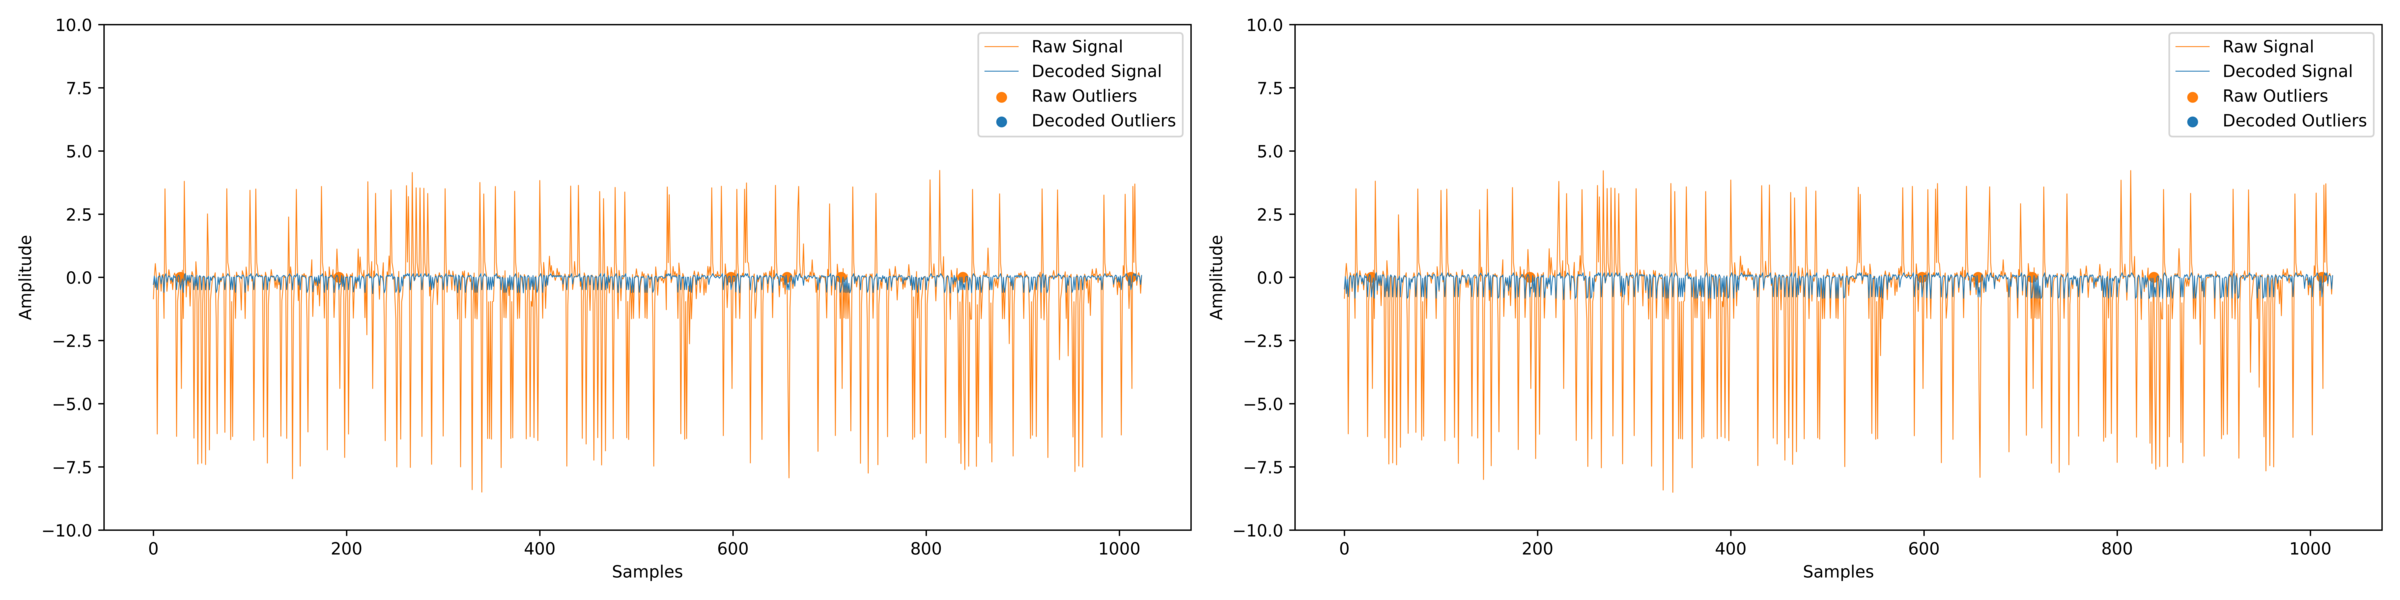
\includegraphics[width=0.8\textwidth]{static/original_vs_decoded_blend_01_resized.png}
    \caption{Signals when blend=0.1}
    \label{fig:signal_01}
\end{figure}
%
When the blend is set to 0.8, the decoded signal captures the patterns and flow of the original signal more accurately, with amplitudes reaching up to approximately $\pm0.5$. This improvement demonstrates that increasing the focus on the mean in the loss function results in an overall better reconstruction of the original signal.
%
\begin{figure}[ht]
    \centering
    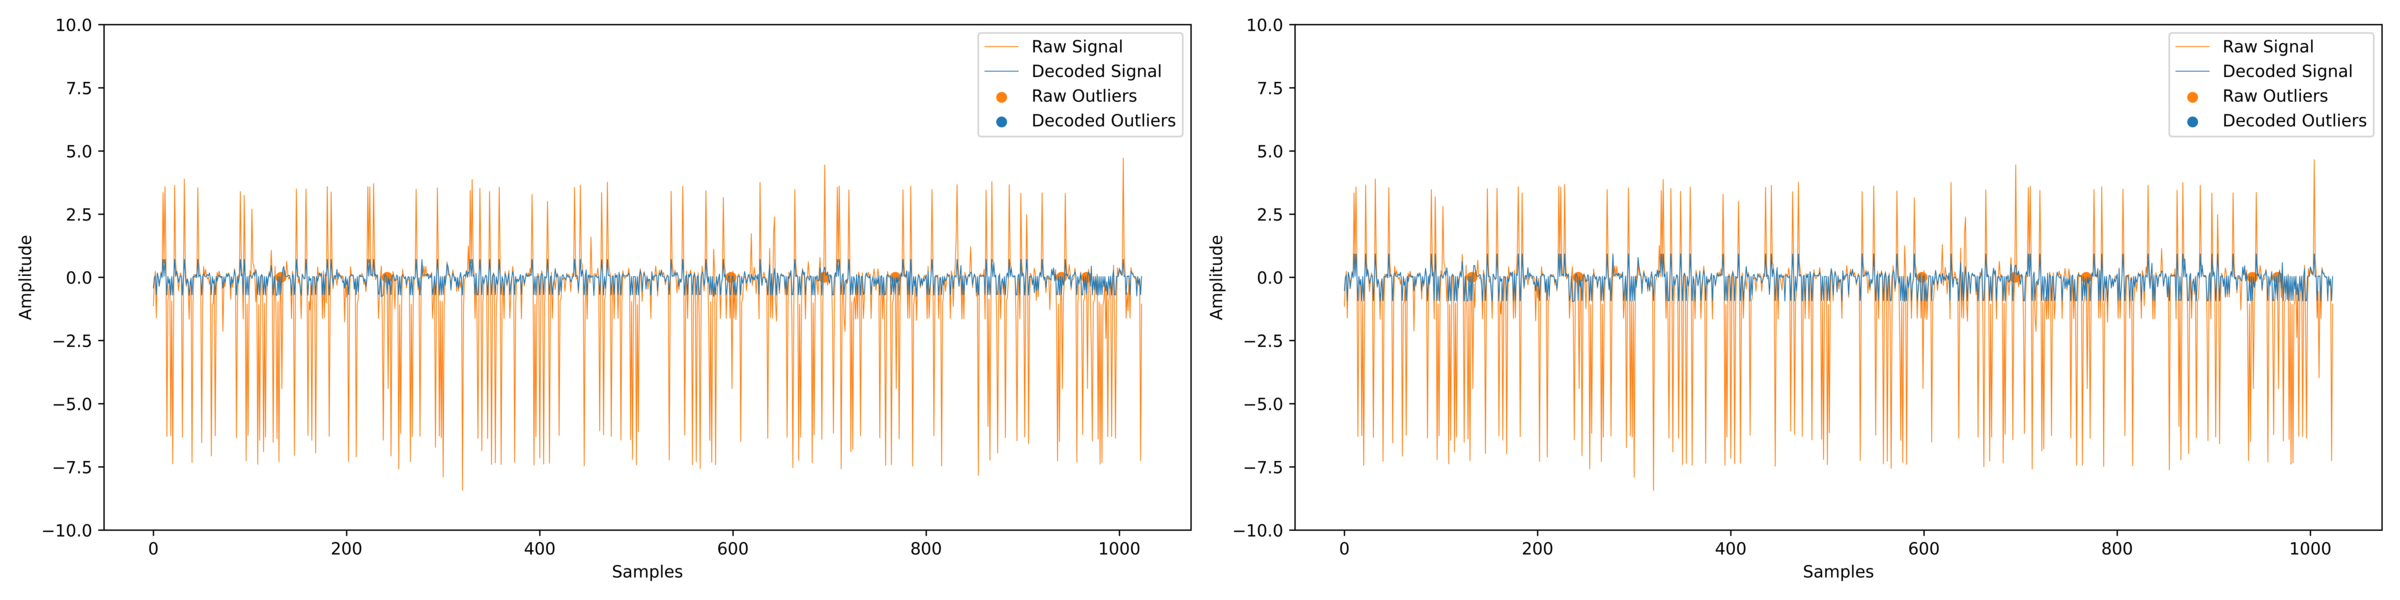
\includegraphics[width=0.8\textwidth]{static/original_vs_decoded_blend_08_resized.png}
    \caption{Signals when blend=0.8}
    \label{fig:signal_08}
\end{figure}
%

\subsubsection{Detrended Signal Comparison} We also analyze the detrended signal using the Theil-Sen estimator. For both the 0.1 and 0.8 blends, the detrended signal trends are nearly flat, indicating minimal differences between the original and decoded signals.
%
\begin{figure}[ht]
    \centering
    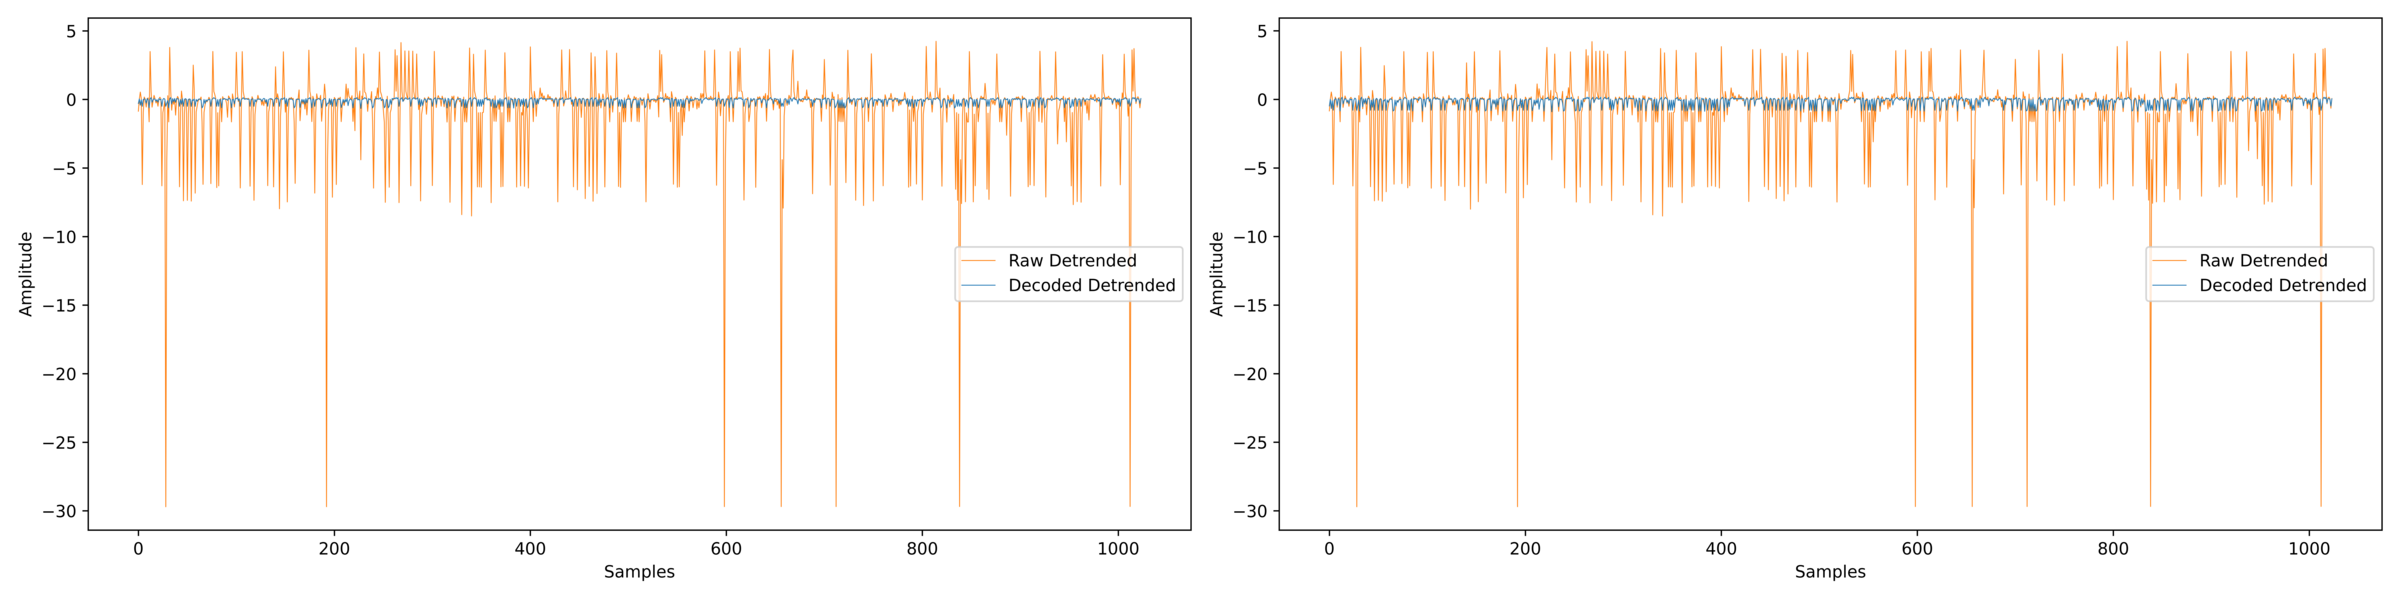
\includegraphics[width=0.8\textwidth]{static/detrended_signal_blend_01_resized.png}
    \caption{Detrended signals when blend=0.1}
    \label{fig:detrended_signal_01}
\end{figure}
%

%
\begin{figure}[ht]
    \centering
    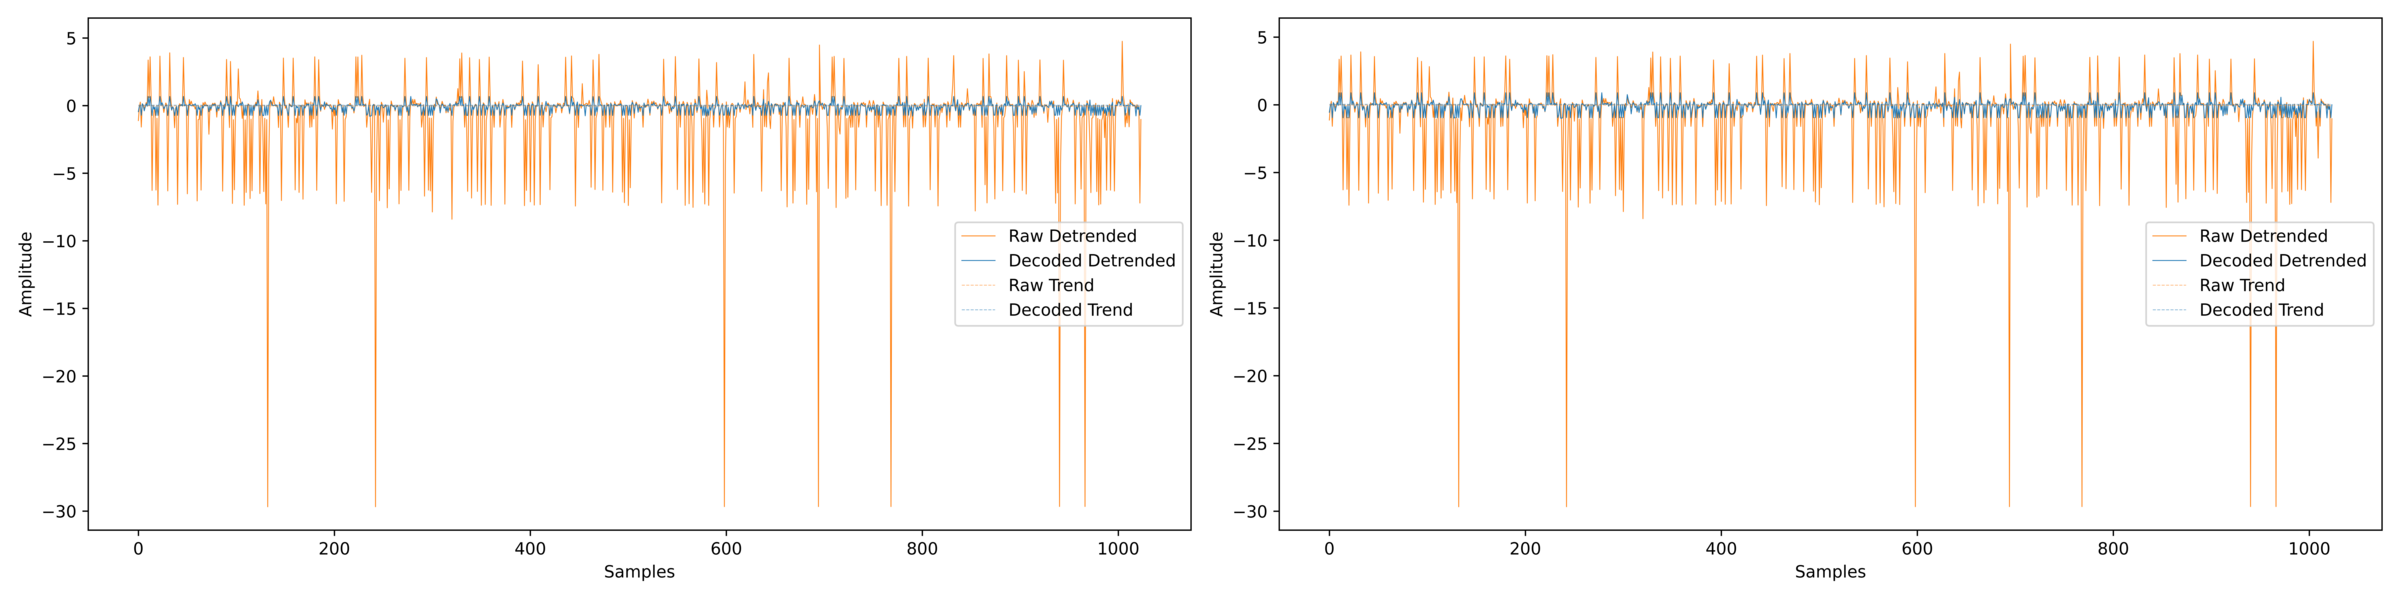
\includegraphics[width=0.8\textwidth]{static/detrended_signal_blend_08_resized.png}
    \caption{Detrended signals when blend=0.8}
    \label{fig:detrended_signal_08}
\end{figure}
%

\subsubsection{RMS Analysis} The root mean square (RMS) analysis provides additional insight into the performance of the autoencoder. When the blend is set to 0.1, the majority of the RMS values are centered around zero, with outliers remaining prominent. This result is acceptable but suggests room for improvement. When the blend is set to 0.8, the RMS shows significant improvement, with a higher count of zeros. The outliers continue to exhibit significant values, but overall, the analysis indicates a better reconstruction.
%
\begin{figure}[ht]
    \centering
    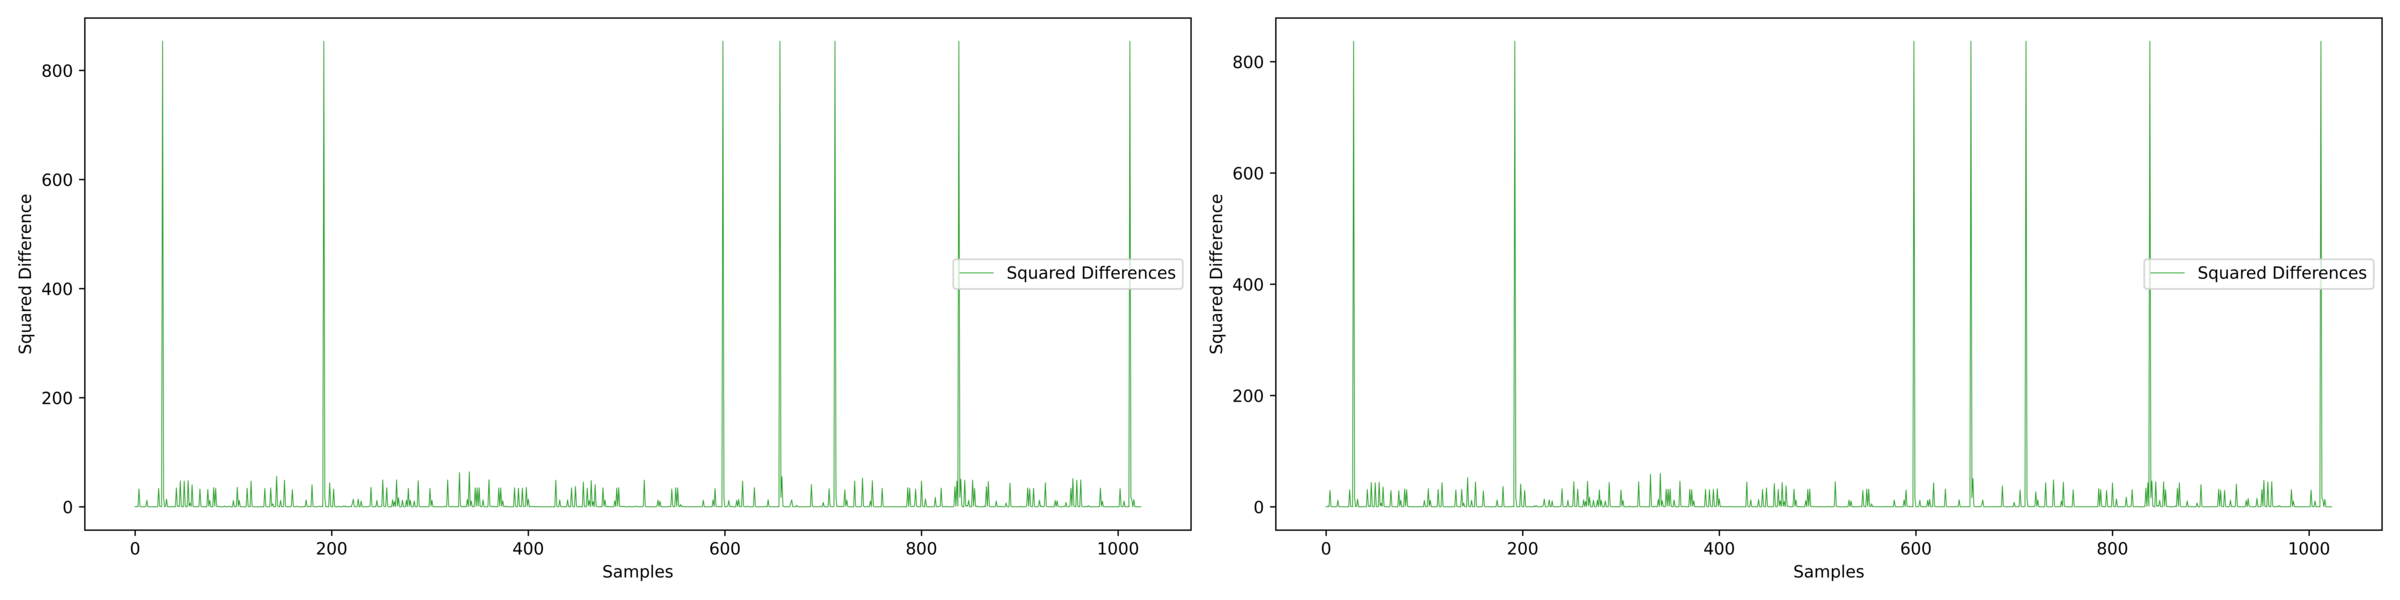
\includegraphics[width=0.8\textwidth]{static/rms_analysis_blend_01_resized.png}
    \caption{RMS analysis when blend=0.1}
    \label{fig:rms_analysis_01}
\end{figure}
%

%
\begin{figure}[ht]
    \centering
    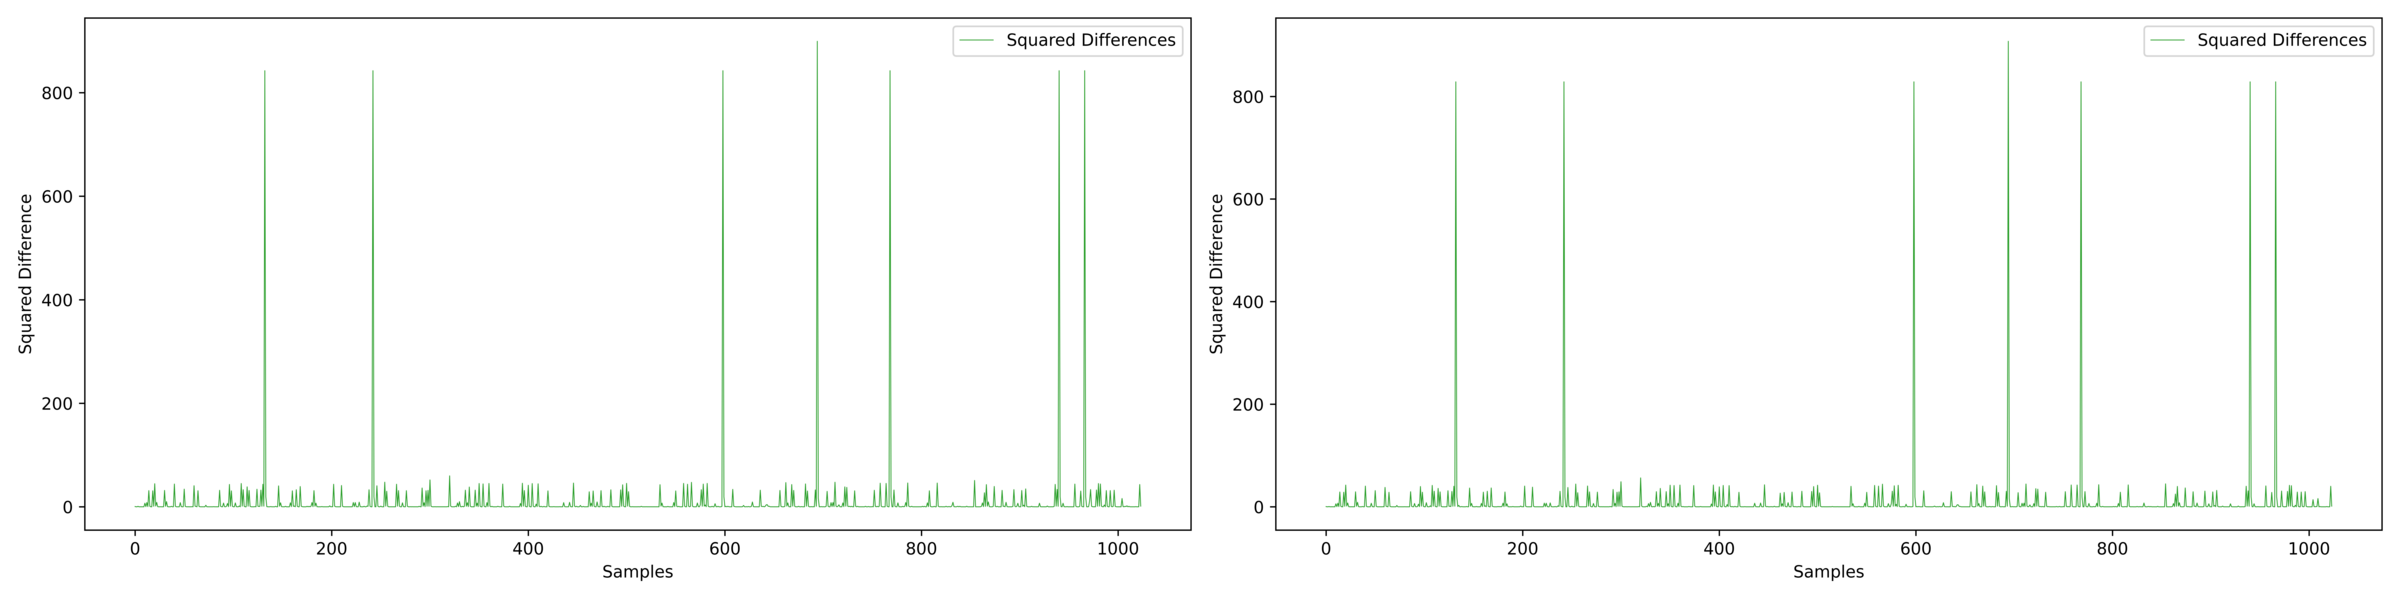
\includegraphics[width=0.8\textwidth]{static/rms_analysis_blend_08_resized.png}
    \caption{RMS analysis when blend=0.8}
    \label{fig:rms_analysis_08}
\end{figure}
%

\subsubsection{Band Analysis} When the blend is set to 0.8, the decoded signal exhibits non-zero values across all bands, indicating a more robust amplitude representation. In some bands, the levels of the decoded signal closely match those of the original signal, suggesting that the model effectively captures the corresponding frequency ranges. In contrast, when the blend is set to 0.1, the distributions of the raw and decoded bands differ significantly. Some bands in the decoded signal are nearly zero, while the raw signal contains substantial values, indicating that the amplitude is not well captured.
%
\begin{figure}[ht]
    \centering
    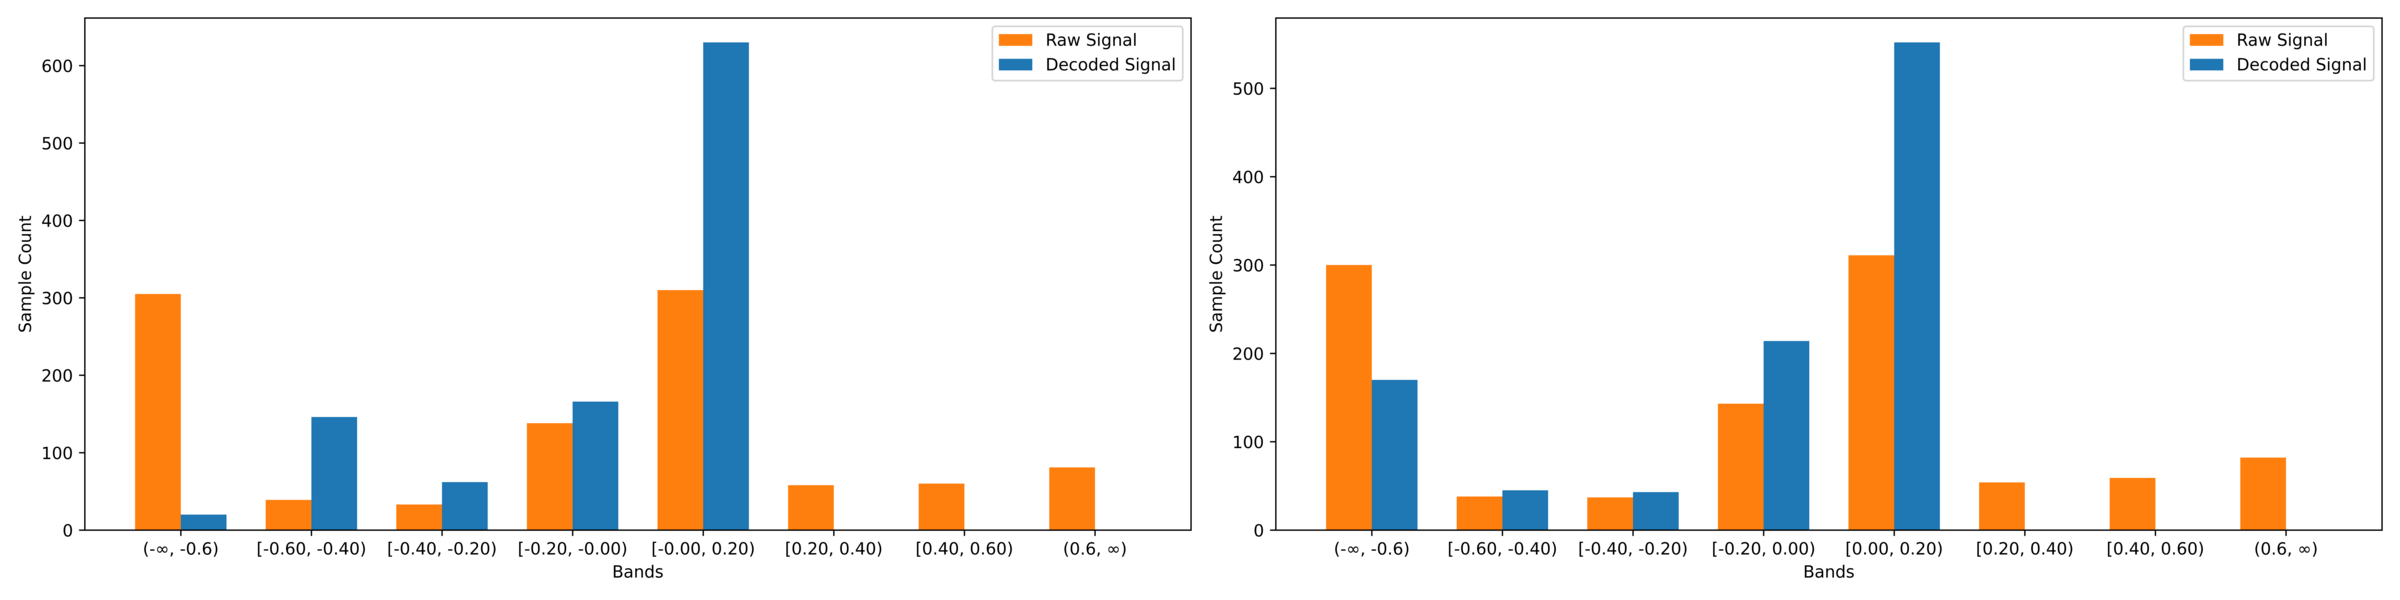
\includegraphics[width=0.8\textwidth]{static/band_analysis_blend_01_resized.png}
    \caption{Band analysis when blend=0.1}
    \label{fig:band_analysis_01}
\end{figure}
%

%
\begin{figure}[ht]
    \centering
    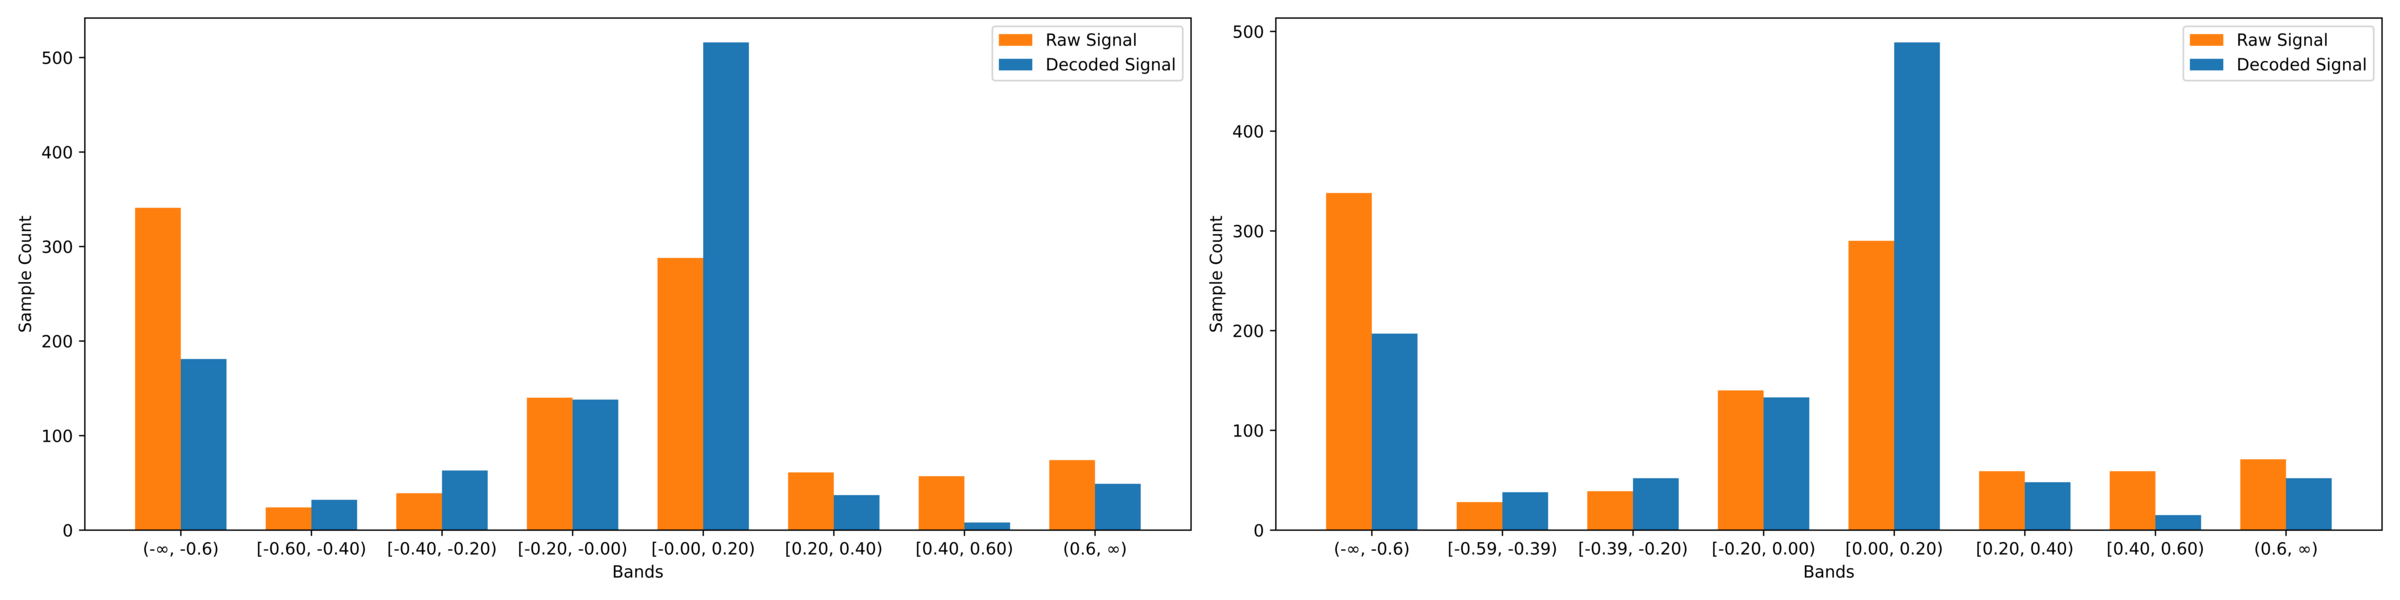
\includegraphics[width=0.8\textwidth]{static/band_analysis_blend_08_resized.png}
    \caption{Band analysis when blend=0.8}
    \label{fig:band_analysis_08}
\end{figure}
%

\subsubsection{Other Metrics}

The performance of the autoencoder is evaluated using various metrics for both blends (0.1 and 0.8). These metrics include band rate differences, zero-crossing rates, RMS values, and Pearson correlation coefficients, calculated as differences between the raw and decoded signals. A smaller difference indicates a closer match to the original signal, which is preferable. Better results are highlighted in blue. Below are the detailed results for each feature and blend setting, showing that the blend with 0.8 is superior.
%
\begin{table}[ht]
    \centering
    \begin{tabular}{l|c|c}
        \hline
        \textbf{Metric} & \textbf{Blend=0.8} & \textbf{Blend=0.1} \\ 
        \hline
        Bands \% $F_1$ & 
        \begin{tabular}[c]{@{}c@{}} 
        \color{blue}{0.4422} \\ 
        1.0 \\ 
        1.0 \\ 
        -0.1232 \\ 
        \color{blue}{0.3420} \\ 
        1.0 \\ 
        1.0 \\ 
        \color{blue}{0.3108} 
        \end{tabular} 
        & 
        \begin{tabular}[c]{@{}c@{}} 
        0.9557 \\ 
        1.0 \\ 
        1.0 \\ 
        \color{blue}{-0.2767} \\ 
        0.7927 \\ 
        1.0 \\ 
        1.0 \\ 
        1.0 
        \end{tabular} \\
        \hline
        
        Bands \% $F_2$ & 
        \begin{tabular}[c]{@{}c@{}} 
        \color{blue}{0.3659} \\ 
        1.0 \\ 
        1.0 \\ 
        \color{blue}{-0.0824} \\ 
        \color{blue}{0.2217} \\ 
        1.0 \\ 
        1.0 \\ 
        \color{blue}{0.2556} 
        \end{tabular} 
        & 
        \begin{tabular}[c]{@{}c@{}} 
        0.4524 \\ 
        1.0 \\ 
        1.0 \\ 
        -0.2741 \\ 
        0.7840 \\ 
        1.0 \\ 
        1.0 \\ 
        1.0 
        \end{tabular} \\
        \hline

        Zero Crossing Rate $F_1$ & 1.3439 & \color{blue}{1.2631} \\ 
 
        Zero Crossing Rate $F_2$ & 1.3334 & \color{blue}{1.0186} \\ 
 
        RMS $F_1$ & \color{blue}{2.8682} & 2.9533 \\ 

        RMS $F_2$ & \color{blue}{2.7980} & 2.8774 \\ 
  
        Pearson Correlation $F_1$ & \color{blue}{0.6527} & 0.6085 \\ 
   
        Pearson Correlation $F_2$ & \color{blue}{0.6610} & 0.6364 \\ 
        \hline
    \end{tabular}
    \caption{Comparison of Metrics for Blends 0.1 and 0.8. Metrics are expressed as differences between Raw and Decoded signals.}
    \label{tab:metrics_comparison}
\end{table}
%



\subsection{Conclusions}

